\documentclass{beamer}
\usetheme{Madrid}

\usepackage[utf8]{inputenc}
\usepackage[T1]{fontenc}
\usepackage[russian]{babel}
\usepackage{animate}
\usepackage{amsfonts}
\usepackage{amssymb}
\usepackage{amsmath}
\usepackage{bm}
\usepackage{adjustbox}
\usepackage{diagbox}
\usepackage{csquotes}
\setbeamertemplate{caption}[numbered]
\graphicspath{{./style/}{./figures/}}
\makeatletter
\defbeamertemplate*{footline}{Dan P theme}
{
  \hbox{
  \begin{beamercolorbox}[wd = 0.5\paperwidth, ht = 2.25ex, dp = 1ex, center]{author in head/foot}
    \usebeamerfont{author in head/foot}
  \end{beamercolorbox}
	
  \begin{beamercolorbox}[wd = 0.48\paperwidth, ht = 2.25ex, dp = 1ex, right]{date in head/foot}
    \usebeamerfont{date in head/foot}\insertshortdate{}\hspace*{2em}
		
\insertframenumber{} / \inserttotalframenumber\hspace*{2ex} 
  \end{beamercolorbox}}
	
  \vskip0pt
}
\makeatother

\begin{document}

\title{Распознавание графиков решения
	одномерного линейного уравнения переноса}

\author{Выполнил: Климов О.\,Д., ФН2--61Б \\ под руководством Галанина М.\,П.}

\date{\today}
\begin{frame}

\titlepage

\end{frame}

\section{Постановка задачи}
\begin{frame}
\frametitle{Постановка задачи}

\begin{block}{Формулировка}
\begin{enumerate}
	\item Необходимо изучить методы численного решения линейного одномерного уравнения переноса. Составить и отладить программу для нахождения численного решения задачи Коши для указанного уравнения. Использовать шесть различных разностных схем. Для всех тестов использовать одинаковую систему тестов.
	
	\item Реализовать модель нейронной сети для распознавания решения уравнения переноса на языке программирования Python. 
	
	\item На основе модели разработать программу, которая по неточному решению возвращает более точное известное решение.
\end{enumerate}
\end{block}
\end{frame}

\begin{frame}
\begin{figure}
	\centering
	\begin{minipage}{0.45\textwidth}
		\centering
		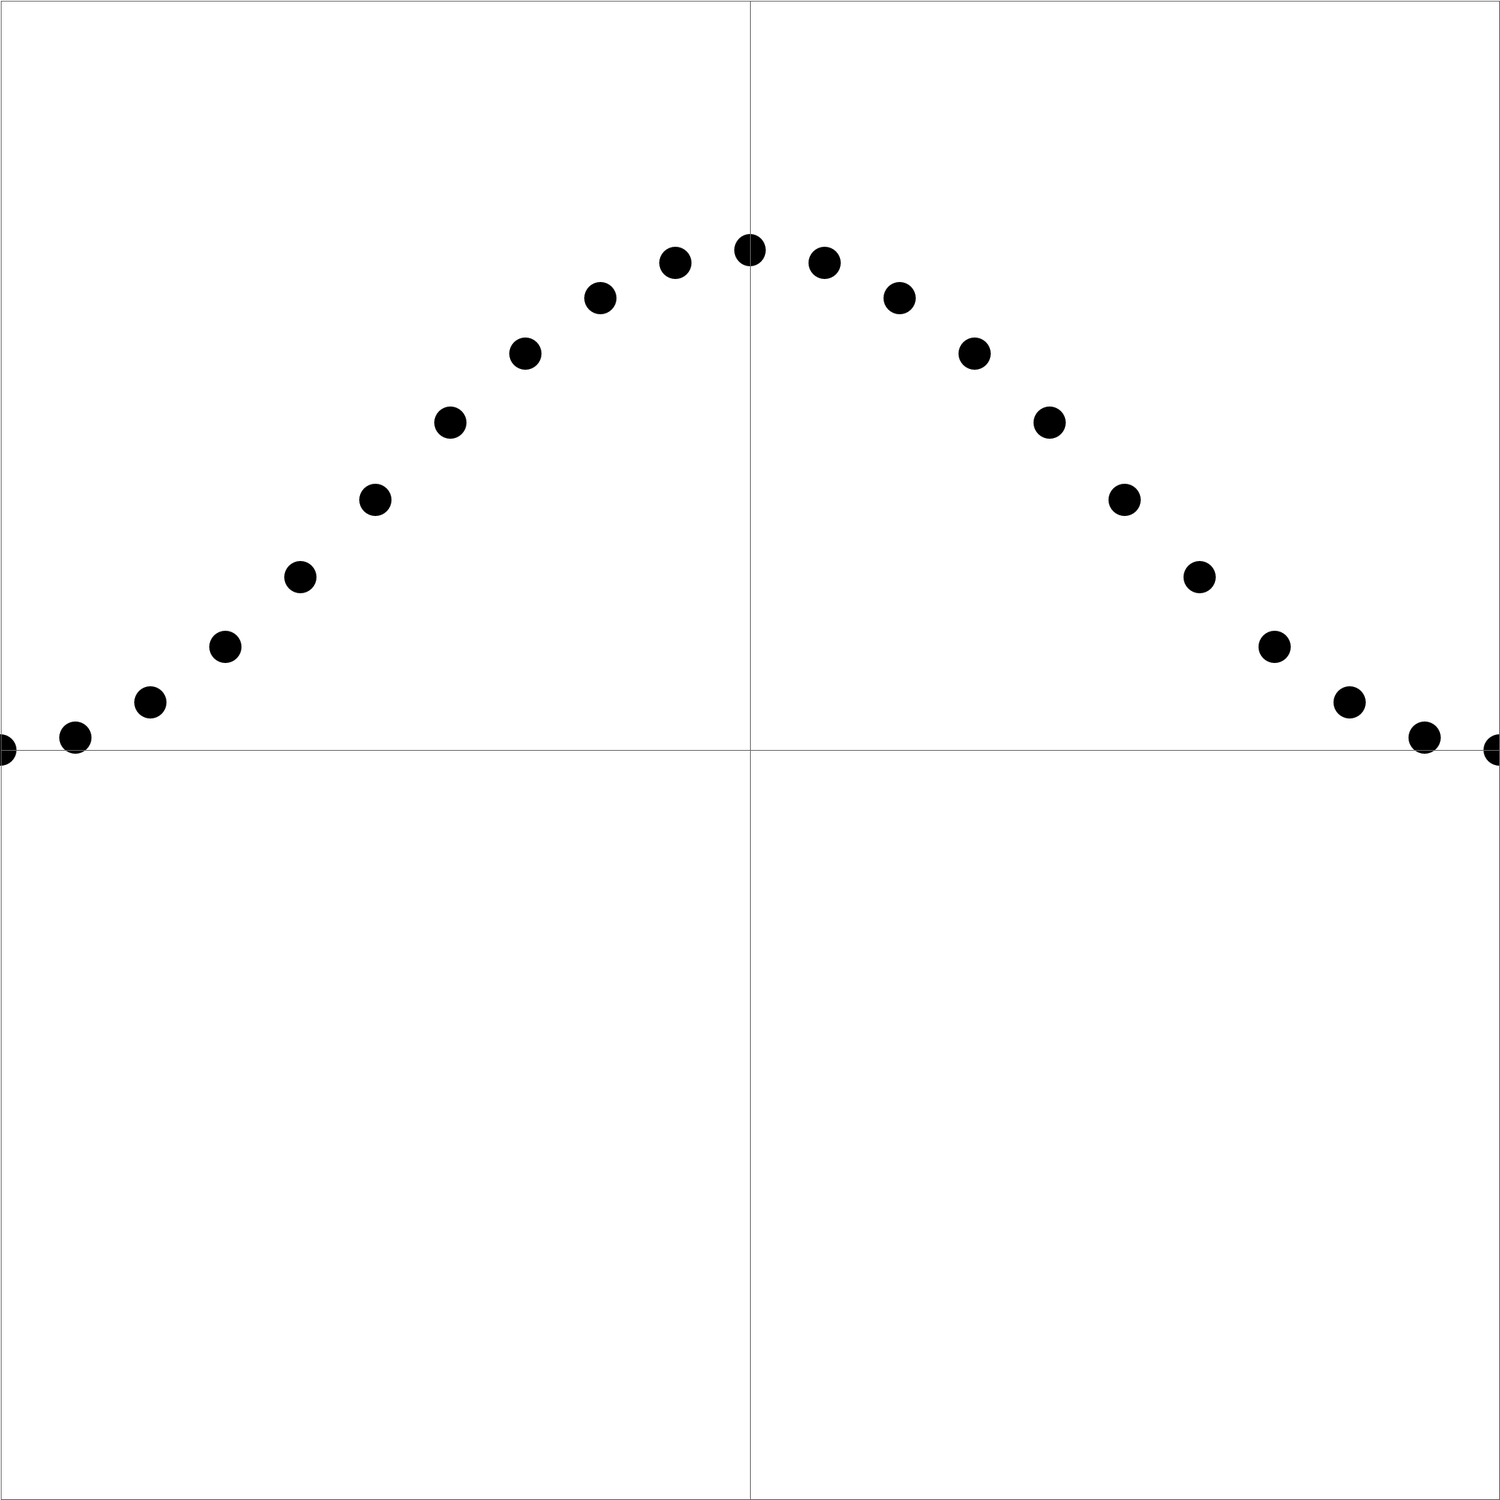
\includegraphics[width=\textwidth]{primer1_1}
		\caption{Численное решение}
		\label{fig:first}
	\end{minipage}\hfill
	\begin{minipage}{0.45\textwidth}
		\centering
		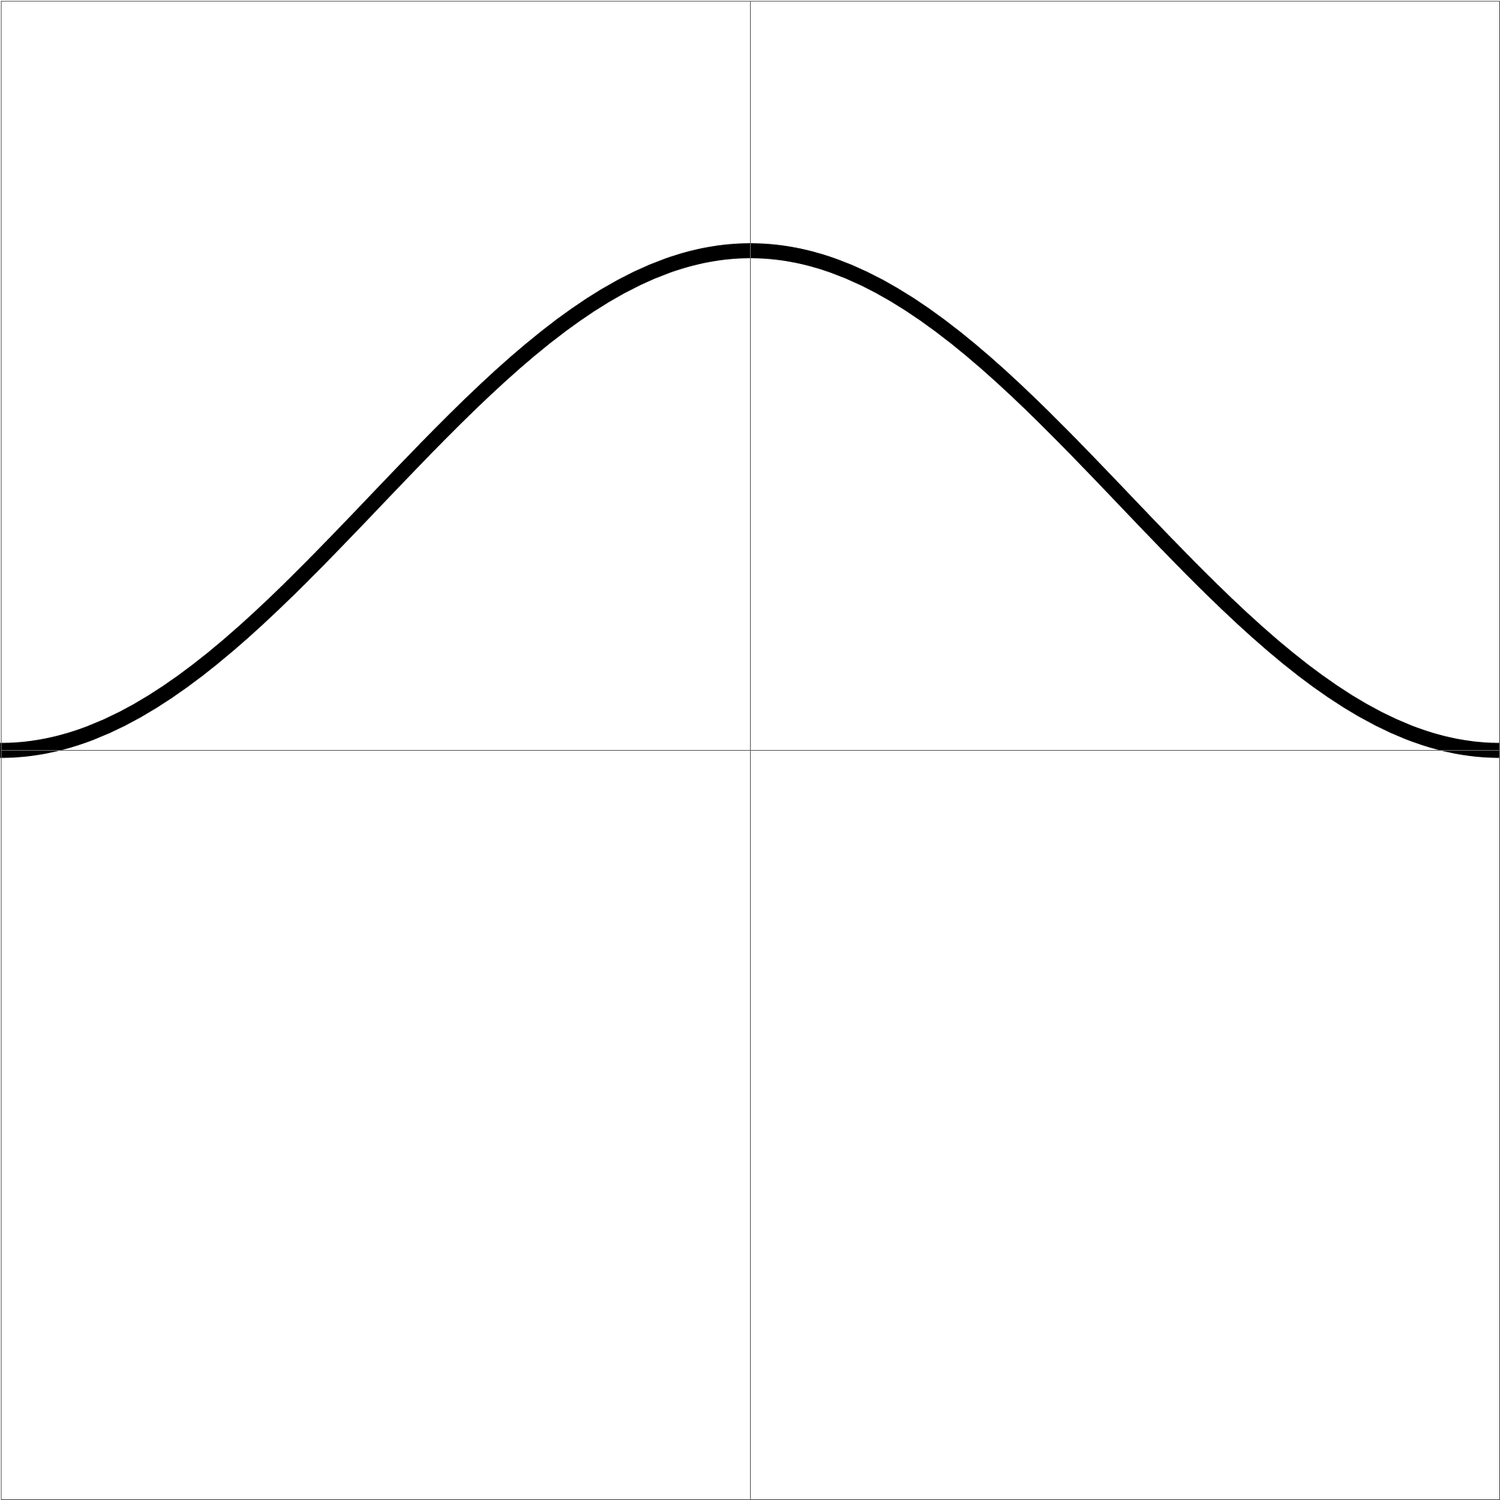
\includegraphics[width=\textwidth]{test4}
		\caption{Улучшенное решение}
		\label{fig:second}
	\end{minipage}
\end{figure}
\end{frame}

\section{Уравнение переноса}
\frametitle{Уравнение переноса}
\begin{frame}
\frametitle{Уравнение переноса}
	\begin{block}{Задача Коши для уравнения переноса}
		\begin{equation}
			\begin{cases}
				\dfrac{\partial u}{\partial t} + a\dfrac{\partial u}{\partial x} = 0, \\
				u(x, 0) = u_0(x),
			\end{cases} 
			\text{где } u = u(x, t), \quad a = const > 0, \quad t \in (0, T), \quad x \in (-\infty, +\infty) .
		\end{equation}
		
		Решение имеет вид $u = u_0(x-at)$ и заключается в сносе неизменного профиля по характеристикам. То есть начальный профиль переносится без искажений с заданной скоростью $a$.
	\end{block}
\end{frame}

\section{Численное решение уравнения переноса}
\begin{frame}
\frametitle{Численное решение уравнения переноса}
\begin{block}{}
	Целью построения методов численного решения данного уравнения является не собственно нахождение его решения, а исследование численного алгоритма на простейшем примере. Аналитическое решение данного уравнения известно и тривиально. При этом в чрезвычайно большое количество математических моделей уравнение переноса входит в качестве составной части.
	
	Разностные схемы в той или иной мере искажают точное решение, например схемы первого порядка, как правило, дают решение «расплывающееся» со временем по пространству. 
	
	
	
	
\end{block}
\begin{block}{}
	Для решения поставленной задачи было рассмотрено 6 схем.
\end{block}
\end{frame}


\begin{frame}
	\begin{block}{Явная схема с левой разностью по 2-м точкам}
	\begin{equation*}
		\widehat{y} = (1 - \gamma) y + \gamma y_{-1}.
		\label{s1}
	\end{equation*}	
	Погрешность аппроксимации схемы: $\psi_h = O(\tau + h)$.
	
	Данная схема является безусловно устойчивой.
		
	\end{block}
	\begin{block}{Неявная схема с левой разностью по 2-м точкам}
	\begin{equation*}
		\widehat{y} = \dfrac{\gamma}{1 + \gamma} \widehat{y}_{-1} + \dfrac{1}{1 + \gamma} y .
		\label{s2}
	\end{equation*}
	
	Погрешность аппроксимации схемы: $\psi_h = O(\tau + h)$.
	
	Данная схема является безусловно устойчивой.
	
	\end{block}
	
	\begin{block}{Явная схема с левой разностью по 3-м точкам}
	
	\begin{equation*}
		\widehat{y} = (1 - \frac{3}{2}\gamma) y + \gamma(2y_{-1} - \frac{1}{2}y_{-2}).
		\label{s3}
	\end{equation*}
	
	Погрешность аппроксимации схемы: 
	$\psi_h = O(\tau + h^2)$.
	
	Схема является безусловно неустойчивой.
		
	\end{block}
\end{frame}


\section{Численное решение уравнения переноса}
\begin{frame}
	\begin{block}{Неявная схема с левой разностью по 3-м точкам}
	\begin{equation*}
		\widehat{y} = \frac{2}{2 + 3 \gamma} y +\frac{\gamma}{2 + 3 \gamma}( 4 \widehat{y}_{-1} -  \widehat{y}_{-2}).
		\label{s4}
	\end{equation*}
	Погрешность аппроксимации схемы: $\psi_h = O(\tau + h)$.
	
	Схема является безусловно неустойчивой.	
		
	\end{block}
	\begin{block}{Схема Лакса}
	\begin{equation*}
		\widehat{y} = \dfrac{(y_{+1} + y_{-1}) - \gamma(y_{+1} - y_{-1})}{2} .
		\label{s5}
	\end{equation*}
	
	Погрешность аппроксимации схемы: $\psi_h = O(\tau + h + \frac{h^2 }{ \tau})$.
	
	Схема устойчива при $\gamma \leq 1 $ и сходится $h^2 \to 0$ быстрее, чем $\tau$.	
		
	\end{block}
	
	\begin{block}{Схема Лакса-Вендрофа}
	\begin{equation*}
		\widehat{y} = y - \gamma(\dfrac{(y_{+1} + y) - \gamma (y_{+1} - y)}{2} -  \dfrac{(y + y_{-1}) - \gamma (y - y_{-1})}{2}).
		\label{s6}
	\end{equation*}
	
	Погрешность аппроксимации схемы: 
	$\psi_h = O(\tau^2 + h^2)$.
	
	Схема устойчива при $\gamma \leq 1 $, а при $\gamma = 1$ схема является точной. 	
		
	\end{block}
\end{frame}


\begin{frame}
	\begin{figure}
		\centering
		\begin{minipage}{0.3\textwidth}
			\centering
			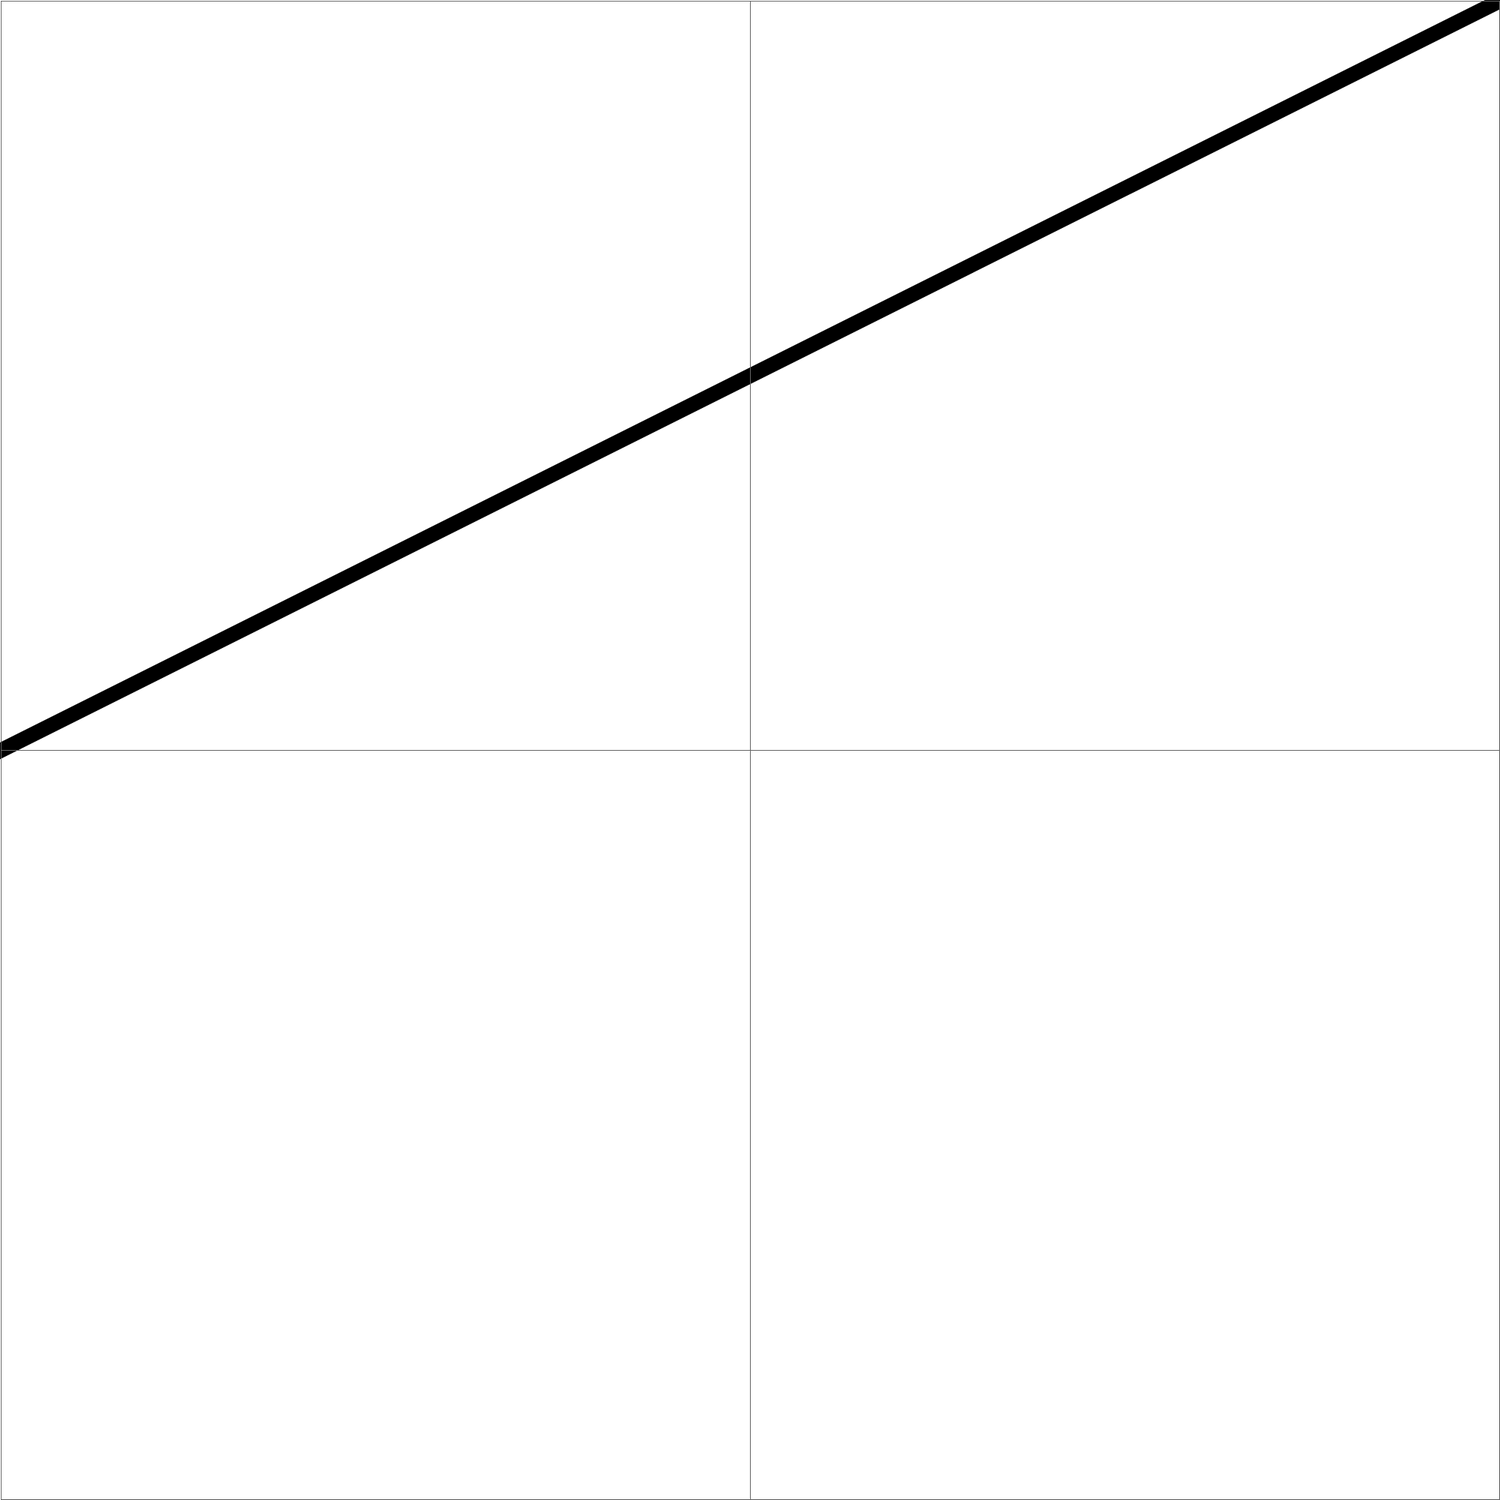
\includegraphics[width=\textwidth]{test1}
			\caption{\parbox{.9\linewidth}{Левый треугольник, \\ $u_0(x) = \frac{x-l_1}{l_2-l_1}$}}
		\end{minipage}\hfill
		\begin{minipage}{0.3\textwidth}
			\centering
			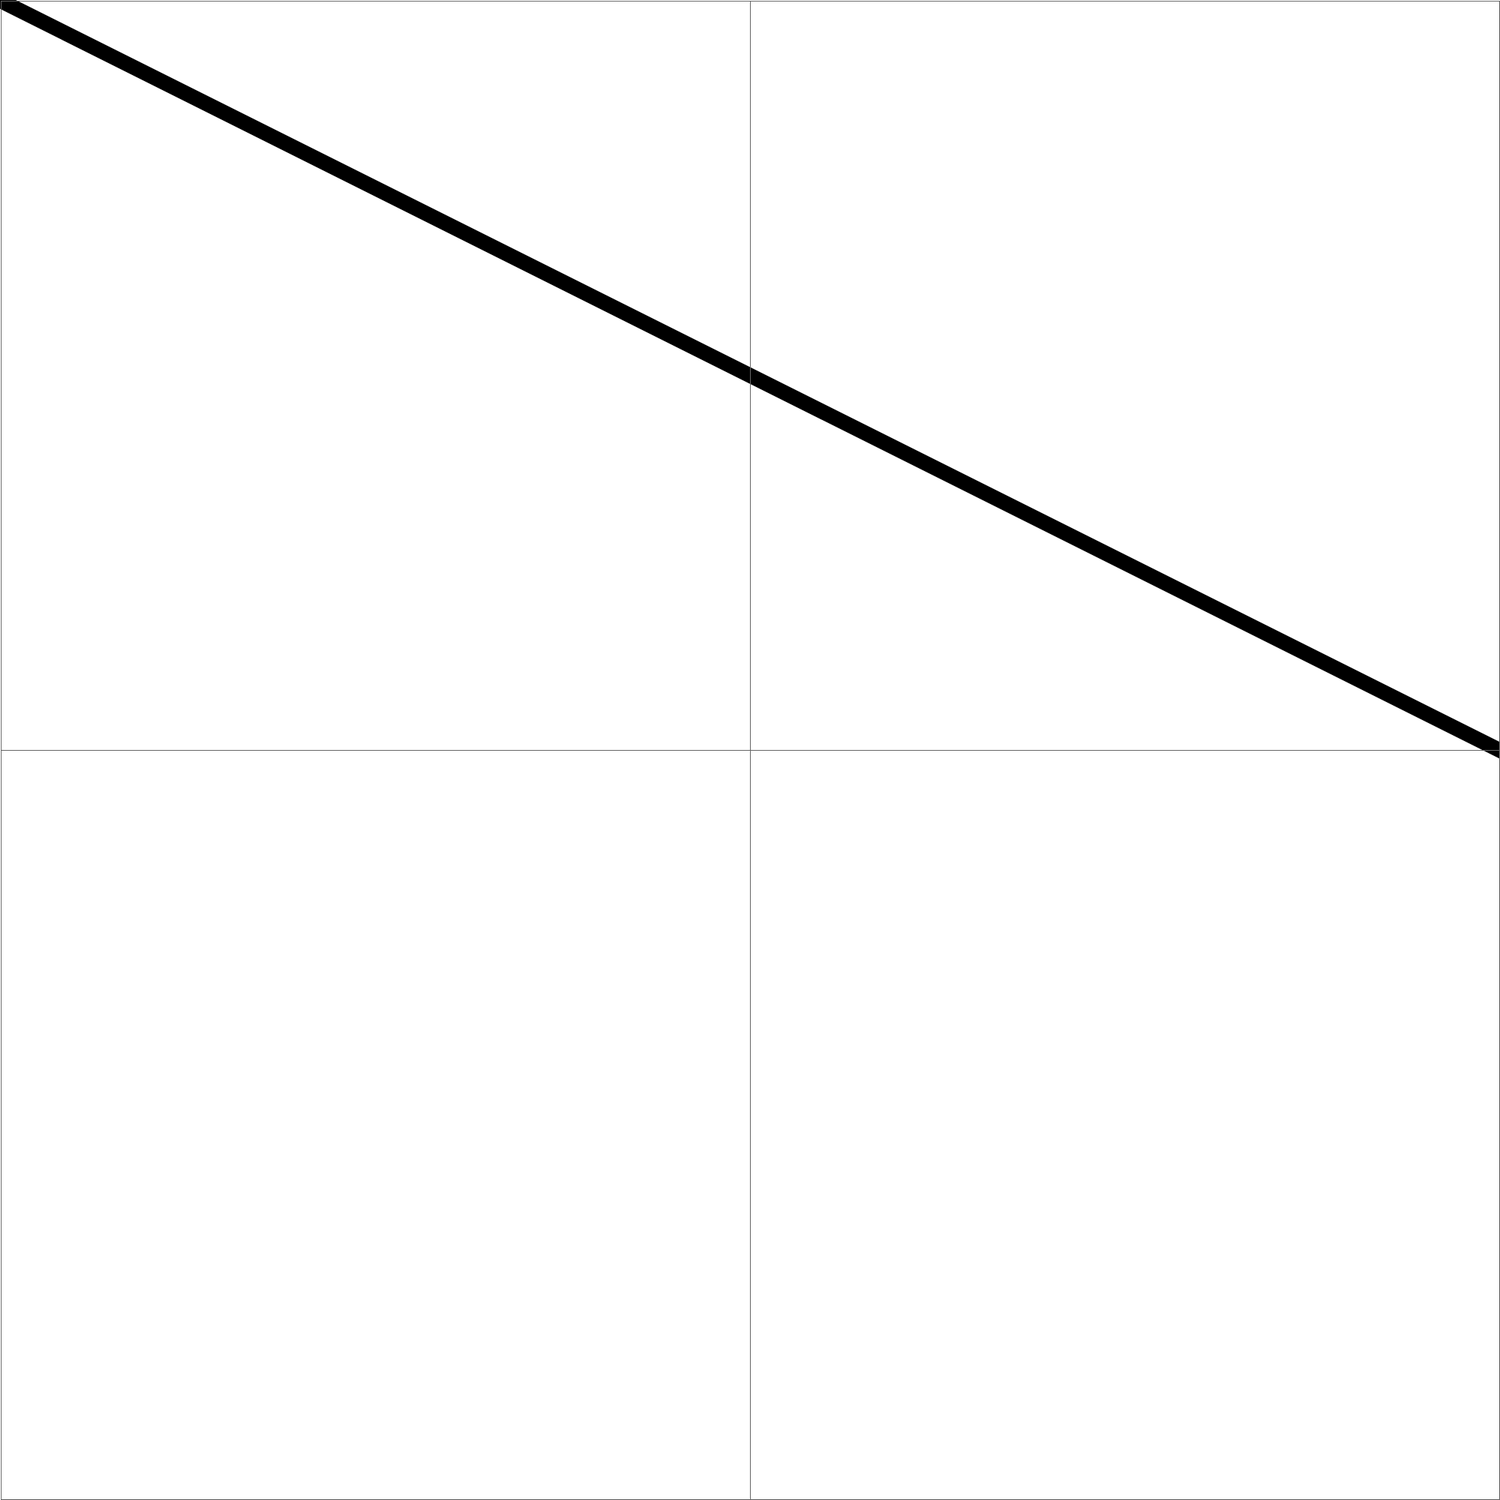
\includegraphics[width=\textwidth]{test2}
			\caption{\parbox{.9\linewidth}{Правый треугольник,\\ $u_0(x) = \frac{l_2-x}{l_2-l_1}$}}
		\end{minipage}\hfill
		\begin{minipage}{0.3\textwidth}
			\centering
			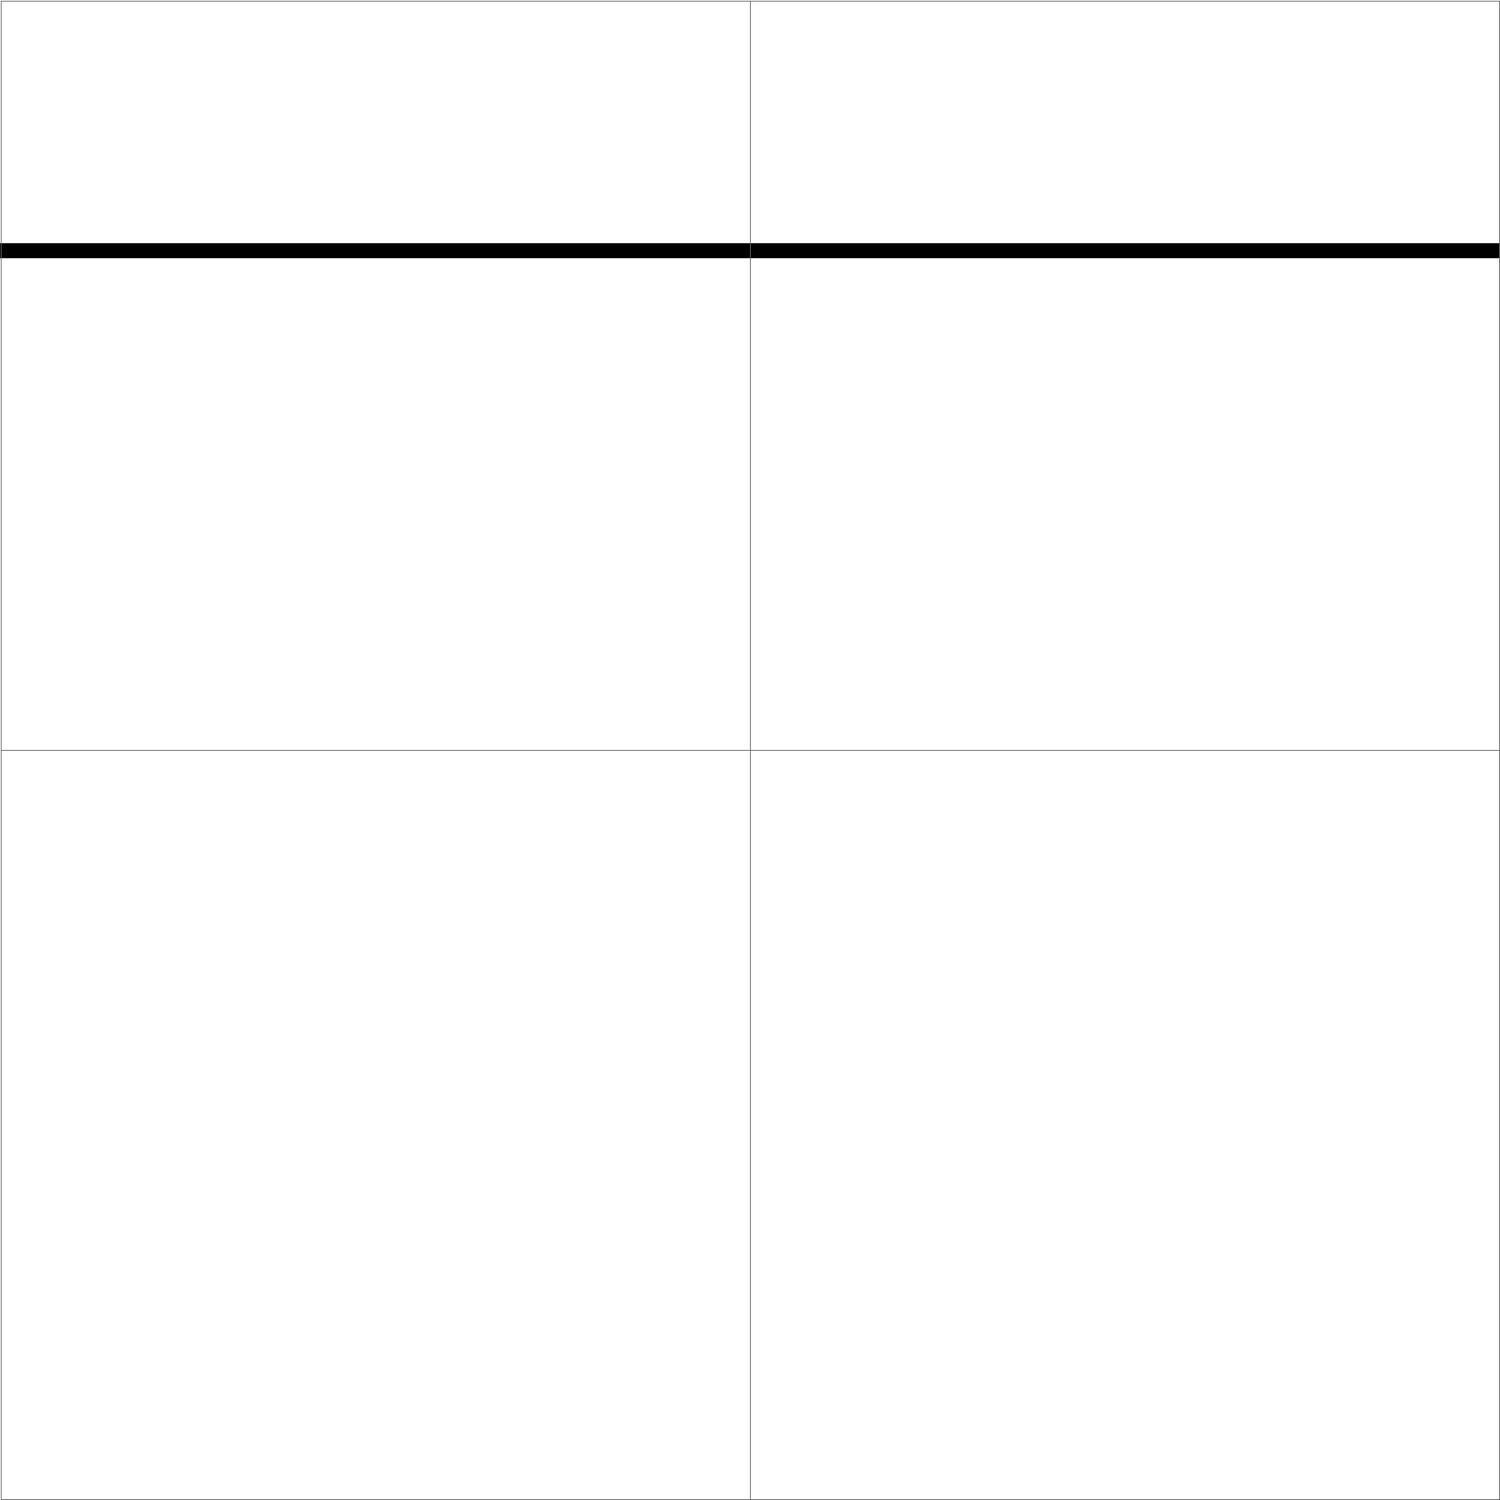
\includegraphics[width=\textwidth]{test3}
			\caption{\parbox{.9\linewidth}{Прямоугольник, \\ $u_0(x) = \frac{2}{3}$}}
		\end{minipage}
	\end{figure}
\end{frame}



\begin{frame}
		\begin{figure}
			\centering
			\begin{minipage}[t]{0.42\textwidth}
				\centering
				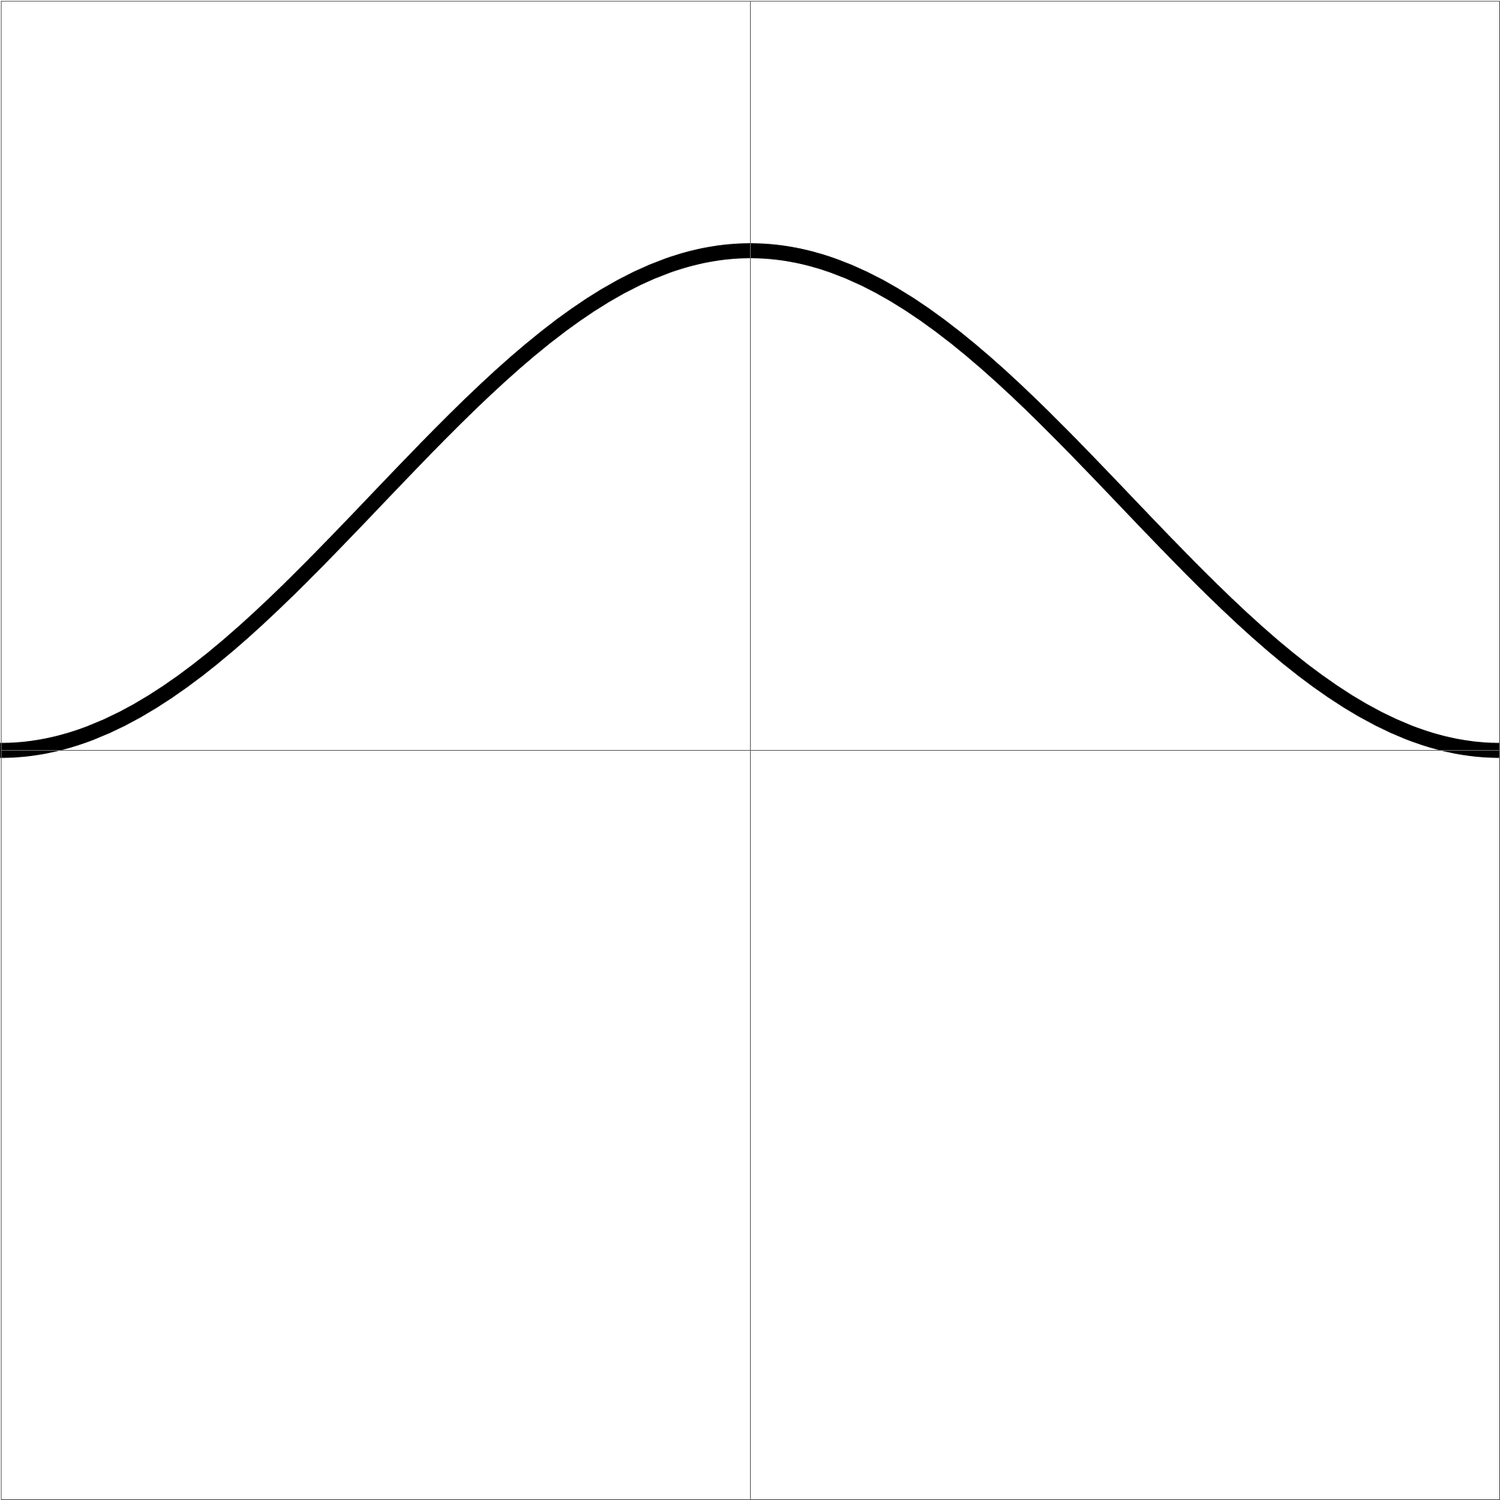
\includegraphics[width=\textwidth]{test4}
				\caption{\parbox{.9\linewidth}{Косинус \\ $u_0(x) = \frac{1}{3} (1 - \cos(\frac{2 \pi (x - l_1)}{l_2 - l_1}))$}}
			\end{minipage}\hspace{0.05\textwidth}
			\begin{minipage}[t]{0.42\textwidth}
				\centering
				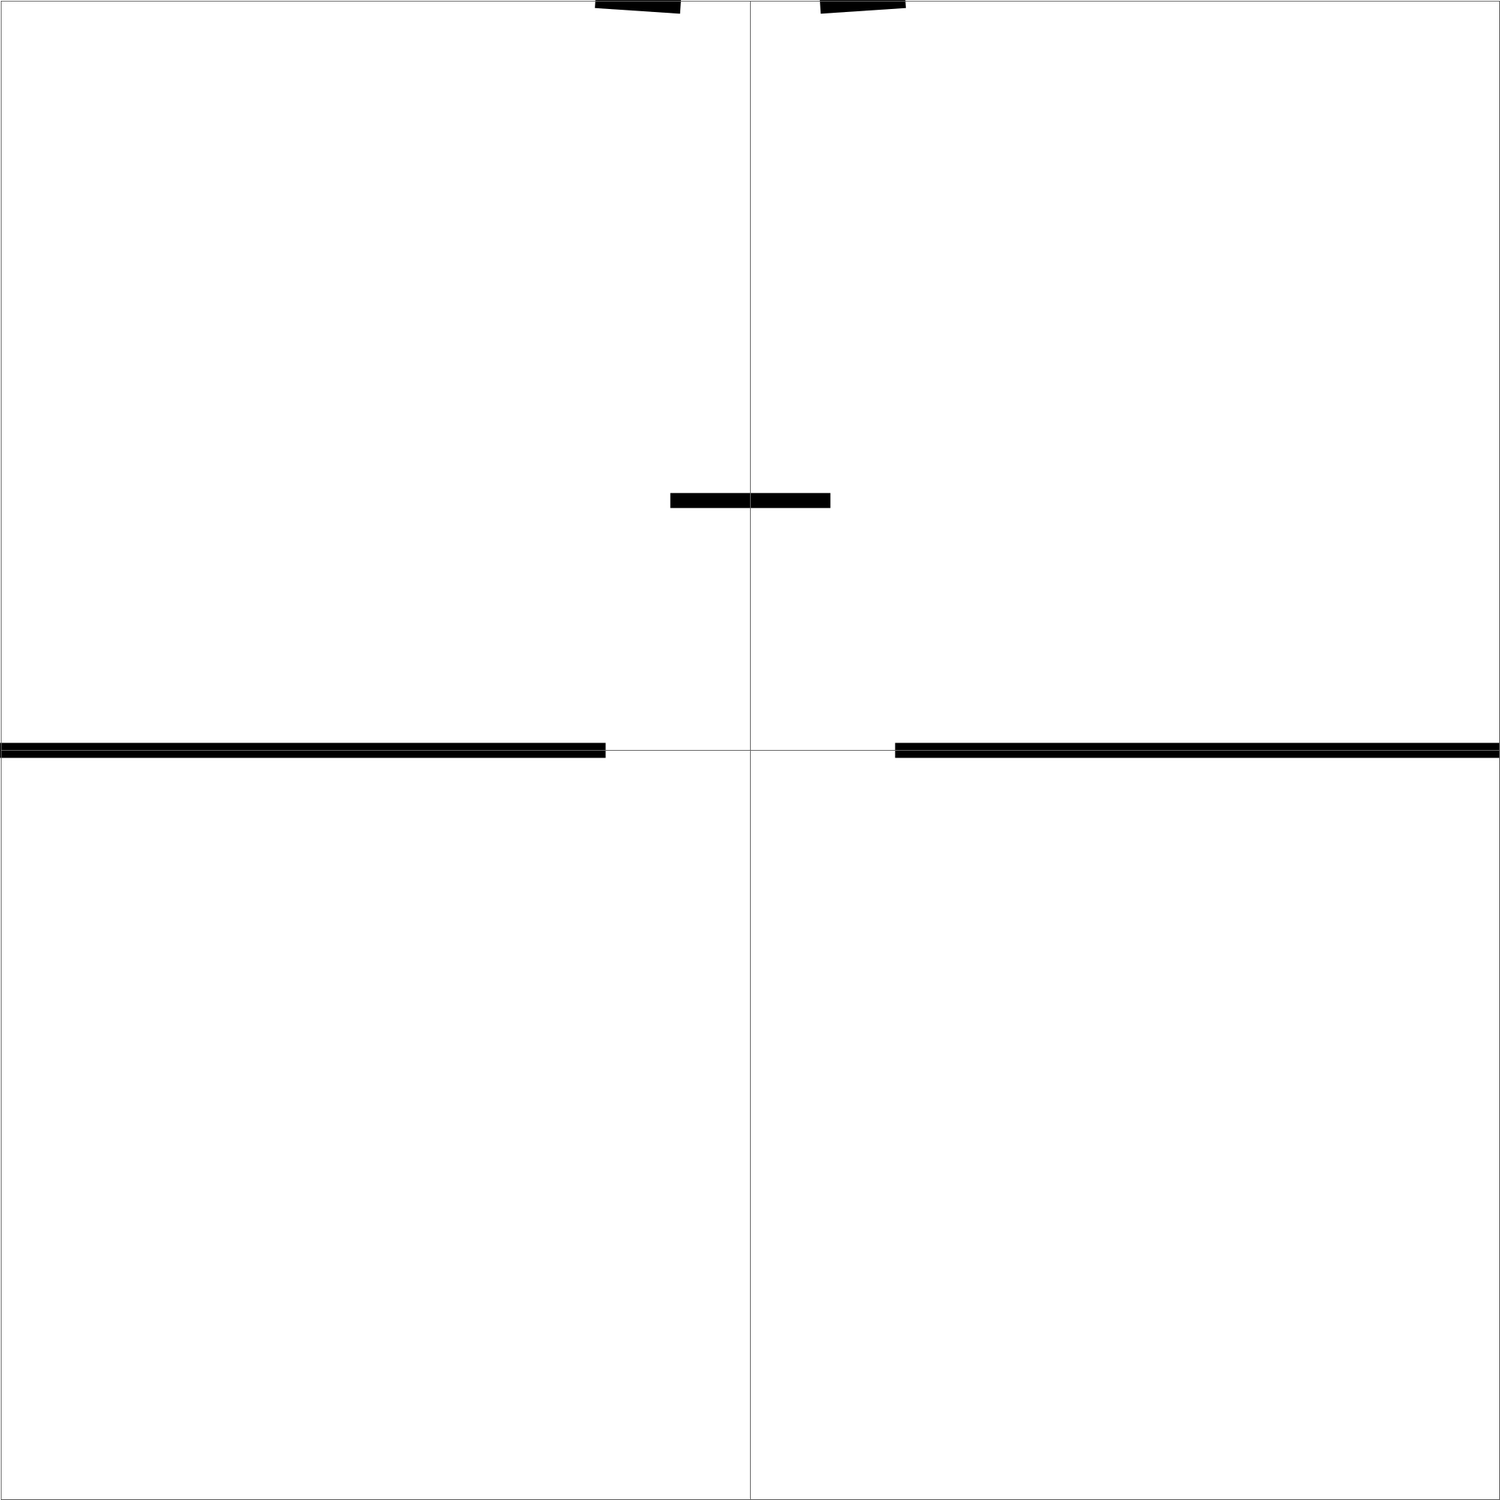
\includegraphics[width=\textwidth]{test5}
				\caption{\parbox{.9\linewidth}{«Зуб» \\[1em]  \adjustbox{scale=0.75}{%
						$u_0(x) =
						\begin{cases}
							-\frac{2}{3} (l_{11} - l_1) (x - l_1) + 1, & l_1 \leq x < l_{11} \\
							\frac{1}{3}, & l_{11} \leq x \leq l_{22} \\
							\frac{2}{3} (l_2 - l_{22}) (x - l_2) + 1, & l_{22} < x \leq l_2
						\end{cases}
						$}}
					}
			\end{minipage}
		\end{figure}
\end{frame}


\section{Результаты реализации схем}
\begin{frame}
	\frametitle{Результаты реализации схем}
	\begin{figure}
		\centering
		\begin{minipage}{0.45\textwidth}
			\centering
			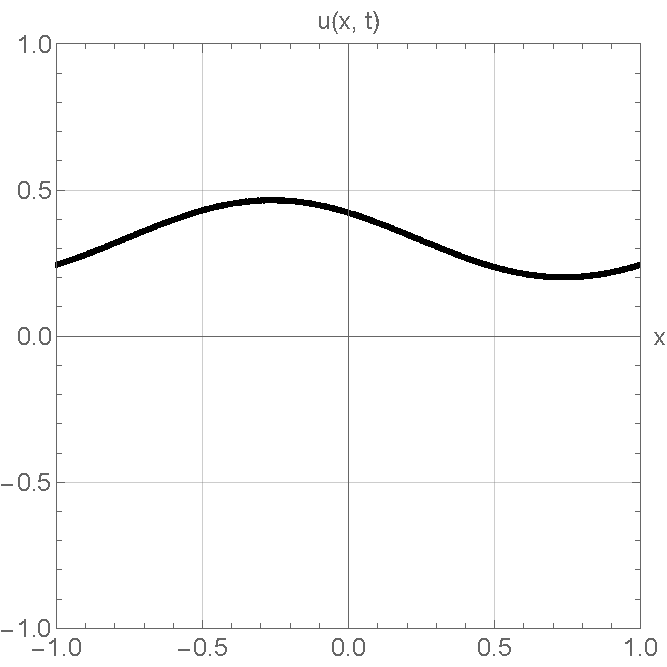
\includegraphics[width=\textwidth]{res1_2}
			\caption{Численное решение}
			\label{fig:first}
		\end{minipage}\hfill
		\begin{minipage}{0.45\textwidth}
			\centering
			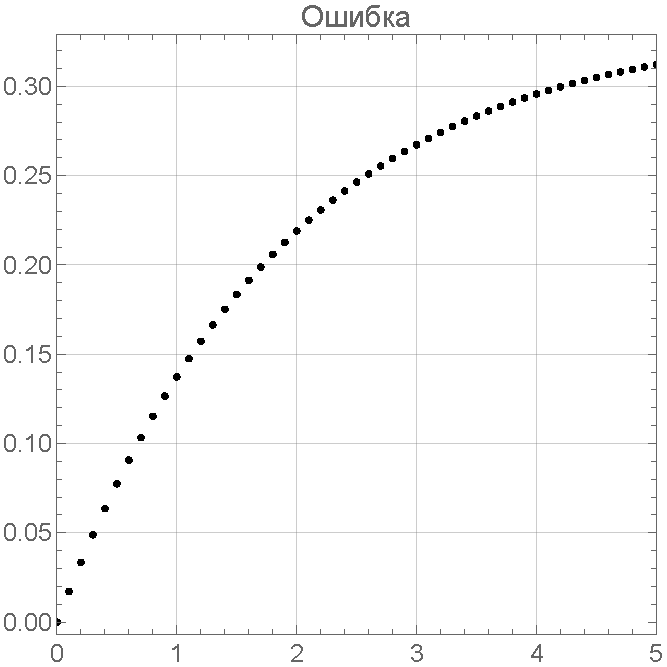
\includegraphics[width=\textwidth]{res1_3}
			\caption{Изменение нормы ошибки}
			\label{fig:second}
		\end{minipage}
	\end{figure}
	\centering Тест косинус по схеме (2), $ t = 2$, при $h = 0.01, \tau = 0.1$
\end{frame}


\begin{frame}
	\frametitle{Результаты реализации схем}
	\begin{figure}
		\centering
		\begin{minipage}{0.45\textwidth}
			\centering
			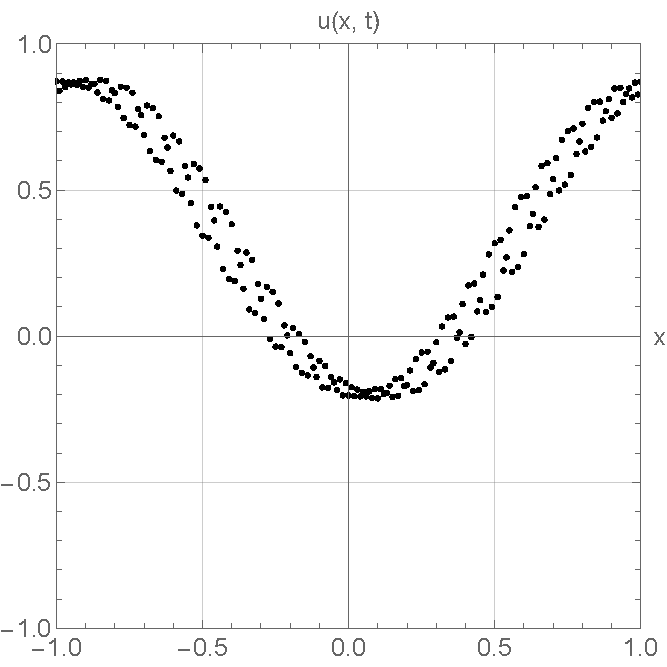
\includegraphics[width=\textwidth]{res2_2}
			\caption{Численное решение}
			\label{fig:first}
		\end{minipage}\hfill
		\begin{minipage}{0.45\textwidth}
			\centering
			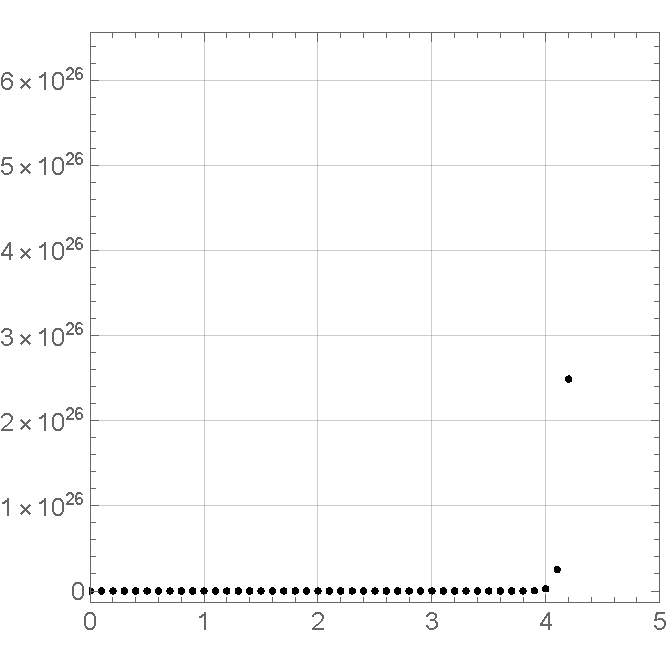
\includegraphics[width=\textwidth]{res2_3}
			\caption{Изменение нормы ошибки}
			\label{fig:second}
		\end{minipage}
	\end{figure}
	\centering Иллюстрация расходимости схемы (1) на тесте косинус, $t = 1.3$, при $h = 0.01, \tau = 0.1$
\end{frame}

\begin{frame}
	\frametitle{Результаты реализации схем}
	\begin{figure}
		\centering
		\begin{minipage}{0.45\textwidth}
			\centering
			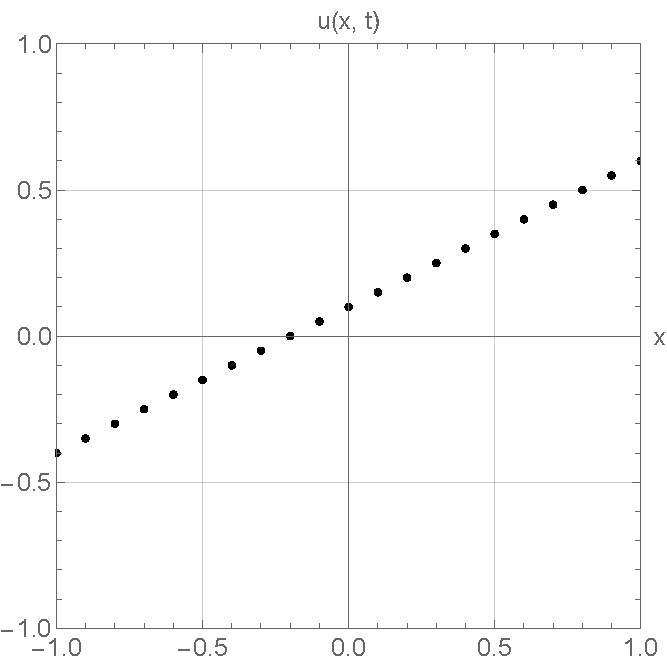
\includegraphics[width=\textwidth]{res3_2}
			\caption{Численное решение}
			\label{fig:first}
		\end{minipage}\hfill
		\begin{minipage}{0.45\textwidth}
			\centering
			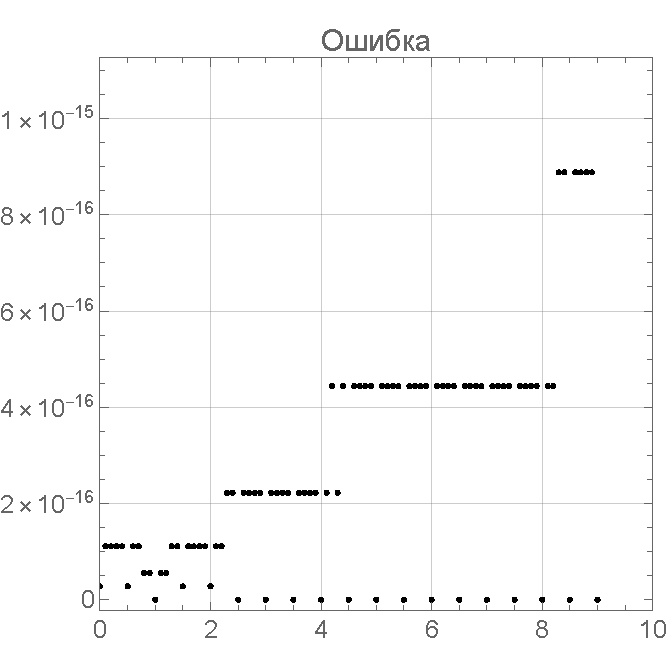
\includegraphics[width=\textwidth]{res3_3}
			\caption{Изменение нормы ошибки}
			\label{fig:second}
		\end{minipage}
	\end{figure}
	\centering Тест левый треугольник по схеме (1), $t = 1.8$ при $h = 0.1, \tau = 0.1$
\end{frame}


\begin{frame}
	\frametitle{Результаты реализации схем}
	\begin{figure}
		\centering
		\begin{minipage}{0.45\textwidth}
			\centering
			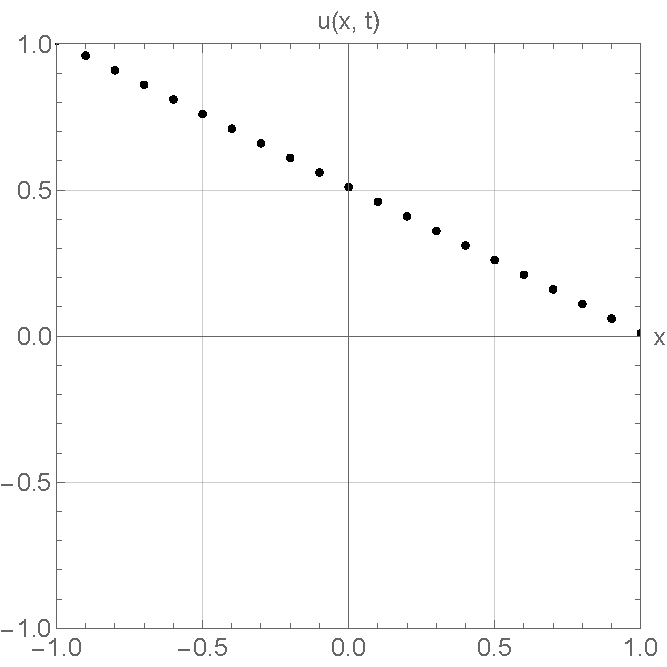
\includegraphics[width=\textwidth]{res5_2}
			\caption{Численное решение}
			\label{fig:first}
		\end{minipage}\hfill
		\begin{minipage}{0.45\textwidth}
			\centering
			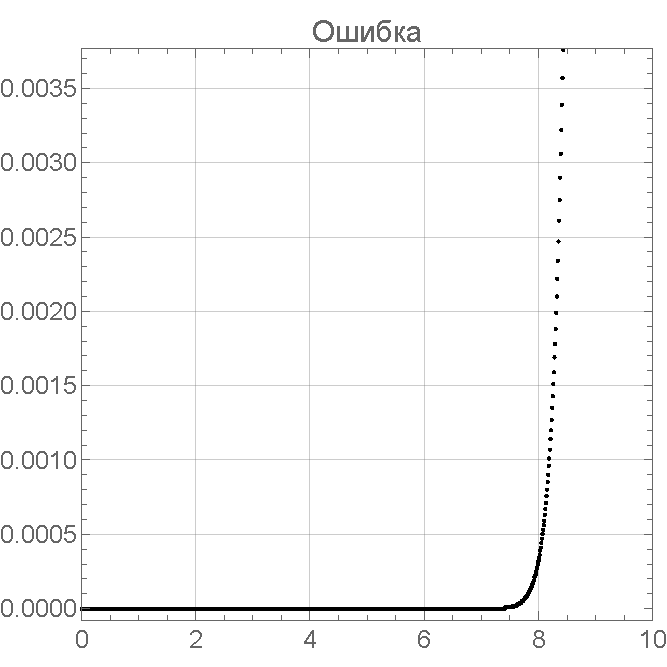
\includegraphics[width=\textwidth]{res5_3}
			\caption{Улучшенное решение}
			\label{fig:second}
		\end{minipage}
	\end{figure}
	\centering Тест правый треугольник по схеме  (6), $ t = 0.5$, при $h = 0.1, \tau = 0.01$
\end{frame}


\begin{frame}
	\frametitle{Результаты реализации схем}
	\begin{table}[ht!]
		\caption{Нормы ошибки разностных схем}
		\centering
		\adjustbox{scale=0.75}{%
			\begin{tabular}{|l|l|l|l|}
				\hline
				\diagbox{$h, \tau$}{Схема}       & Явная ЛДР 1-го пор.     & Неявная ЛДР 1-го пор.  & Явная ЛДР 2-го пор.    \\ \hline
				\textbf{$h = 0.1, \tau = 0.1$}   & $ 4.44 \cdot 10^{-16}$  & $ 4.2 \cdot 10^{-2}$ &  $1632$   \\ \hline
				\textbf{$h = 0.1, \tau = 0.01$}  & $5.2 \cdot 10^{-2} $      & $6.7 \cdot 10^{-2} $ &  $1229$ \\ \hline
				\hline
				\diagbox{$h, \tau$}{Схема}       & Неявная ЛДР 2-го пор.   & Лакса                  & Лакса-Вендрофа          \\ \hline
				\textbf{$h = 0.1, \tau = 0.1$}   & $10^{18}$               & $9.1 \cdot 10^{-2} $   & $4.46 \cdot 10^{-16} $  \\ \hline
				\textbf{$h = 0.01, \tau = 0.1$}  & $10^{54}$               & $3.3 \cdot 10^{32} $  	& $5.4 \cdot 10^{34} $    \\ \hline
			\end{tabular}
		}
		\label{tab1}
	\end{table}
\end{frame}

\section{Описание алгоритма сверточной нейронной сети}
\begin{frame}
	\frametitle{Алгоритм сверточной нейронной сети}	
	\begin{block}{Достоинства модели}
		Сверточная нейронная сеть обладает способностью улавливать пространственные взаимосвязи на изображении, то есть распознавать объекты независимо от их положения и размера на изображении. Весами(настраиваемыми параметрами) являются матрицы(фильтры), которые используется целиком для всего изображения, благодаря чему модель требует меньшее количество времени для обучения.
	\end{block}
	Алгоритм сверточной нейронной сети состоит из следующих этапов:
	\begin{block}{Этап 1: Входные данные (входной слой)}
		Пусть дано черно-белое изображение размером $(n, n)$ пикселей. Изображение представляется в виде матрицы $A$ той же размерности, а каждый элемент принимает значение яркости соответствующего пикселя.
	\end{block}
\end{frame}



\begin{frame}
	\frametitle{Алгоритм сверточной нейронной сети}	
	\begin{block}{Этап 2: Извлечение признаков (Слой свертки)}
		Выбирается матрица $F$, являющаяся по своей сути фильтром. Производится операция свертки для входной матрицы $A$. 
		
		Получаем новую матрицу $M = A * F$
	\end{block}	
	
	\begin{figure}[p]
		\centering
		
		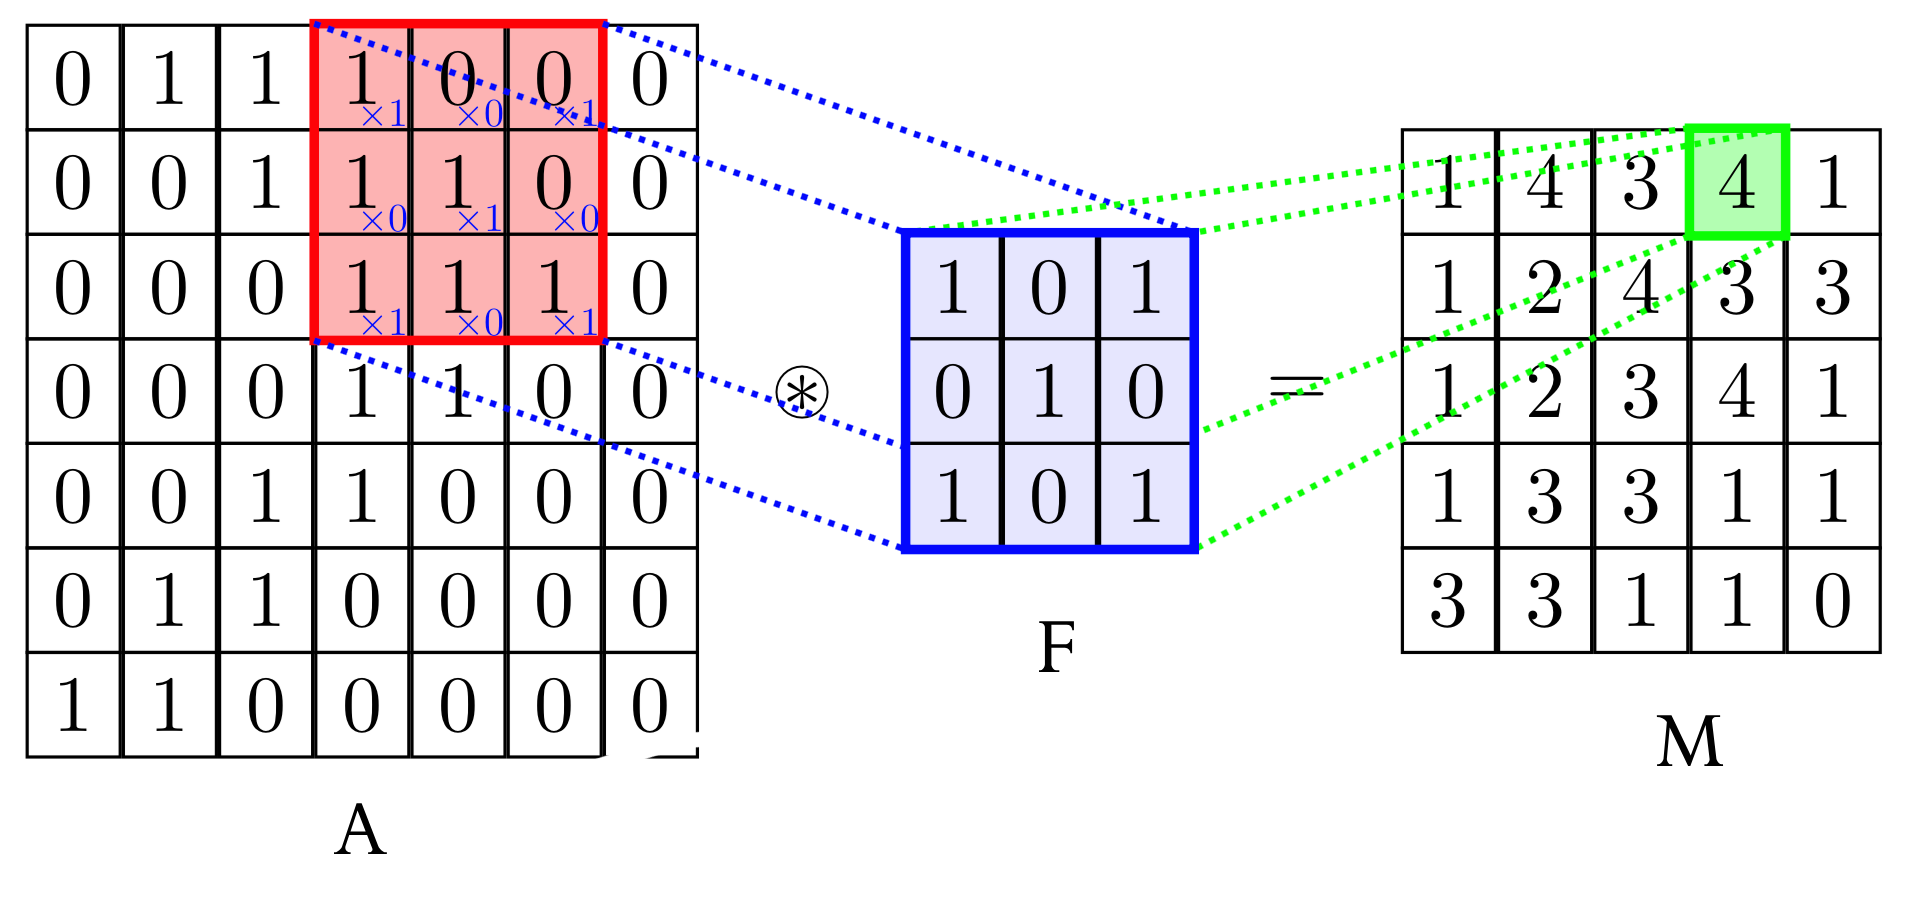
\includegraphics[width=0.7\textwidth]{conv1.png}
		\caption{Иллюстрация операции свертки}
	\end{figure}
\end{frame}



\begin{frame}
	\frametitle{Алгоритм сверточной нейронной сети}	
	\begin{block}{Этап 3: Отбор признаков (Слой пуллинга)}
		Разбиваем матрицу $M$ на подматрицы равной размерности и заменяем ее наибольшими элементами соответствующих подматриц. Данный этап позволяет уменьшить размерность последующих матриц, получаемых после операции свертки. Это приводит к уменьшению количества параметров в сети и ускорению обучения, а также уменьшает эффект переобучаемости нейросети.
	\end{block}	
	\begin{block}{Этап 4: Классификация (полносвязный слой)}
		Матрица $M$ преобразовывается в вектор, путем последовательного соединения строк, после чего осуществляем алгоритм перцептрона. 
	\end{block}	
	
\end{frame}


\section{Задача распознавания}
\begin{frame}
	\frametitle{Задача распознавания решения}	
	\begin{block}{Формулировка}
		Пусть дано изображение графика решения $u(x, t)$ в определенной области. Пусть это изображение имеет искажения, в нашем случае --- погрешность решения. Основываясь на нем, необходимо с определенной точностью определить вид функции $u(x, t)$.
	\end{block}	
	
	\begin{block}{Ограничения}
		В силу конечности множества вариантов ответа нейронной сети, введем ограничения задачи:
		\begin{enumerate}
			\item Рассмотрим решения, относящиеся исключительно к рассмотренным теста
			\item Будем рассматривать решения на определенной сетке до некоторого $T$
			\item Будем рассматривать изображения определенной размерности
		\end{enumerate}	
	\end{block}	
\end{frame}


\begin{frame}
	\frametitle{Краткий обзор библиотек машинного обучения}
	Библиотека TensorFlow
	\begin{block}{Достоинства}
		\begin{enumerate}
			\item Высокая производительность
			\item Статический граф вычислений
			\item Наиболее полный набор инструментов и функций
			\item Представление данных в \enquote{тензорах}, что обеспечивает высокую степень абстракции для операций.
			
			
			
			
			
			
		\end{enumerate}
	\end{block}
	
	\begin{block}{Недостатки}
		\begin{enumerate}
			\item Сложность изучения всех возможностей библиотеки, в связи отсутствием русскоязычной литературы
			\item Большой объем файлов и их зависимостей, из-за чего библиотека часто \enquote{ломается}
			
		\end{enumerate}
	\end{block}	
\end{frame}

\section{Программа улучшения решения уравнения переноса}
\begin{frame}
\frametitle{Программа улучшения решения уравнения переноса}
\begin{block}{Идея алгоритма}
	Чтобы распознать на изображении определенное решение уравнения, необходимо произвести расчет модели нейронной сети и получить ее ответ. Этим ответом будет метка, которая была назначена во время обучения каждому решению. Зная метку, можно поставить в соответствие исходное для обучения изображение, которое и будет являться улучшенным решением. 
\end{block}
		\begin{figure}
			\centering
			\begin{minipage}{0.35\textwidth}
				\centering
				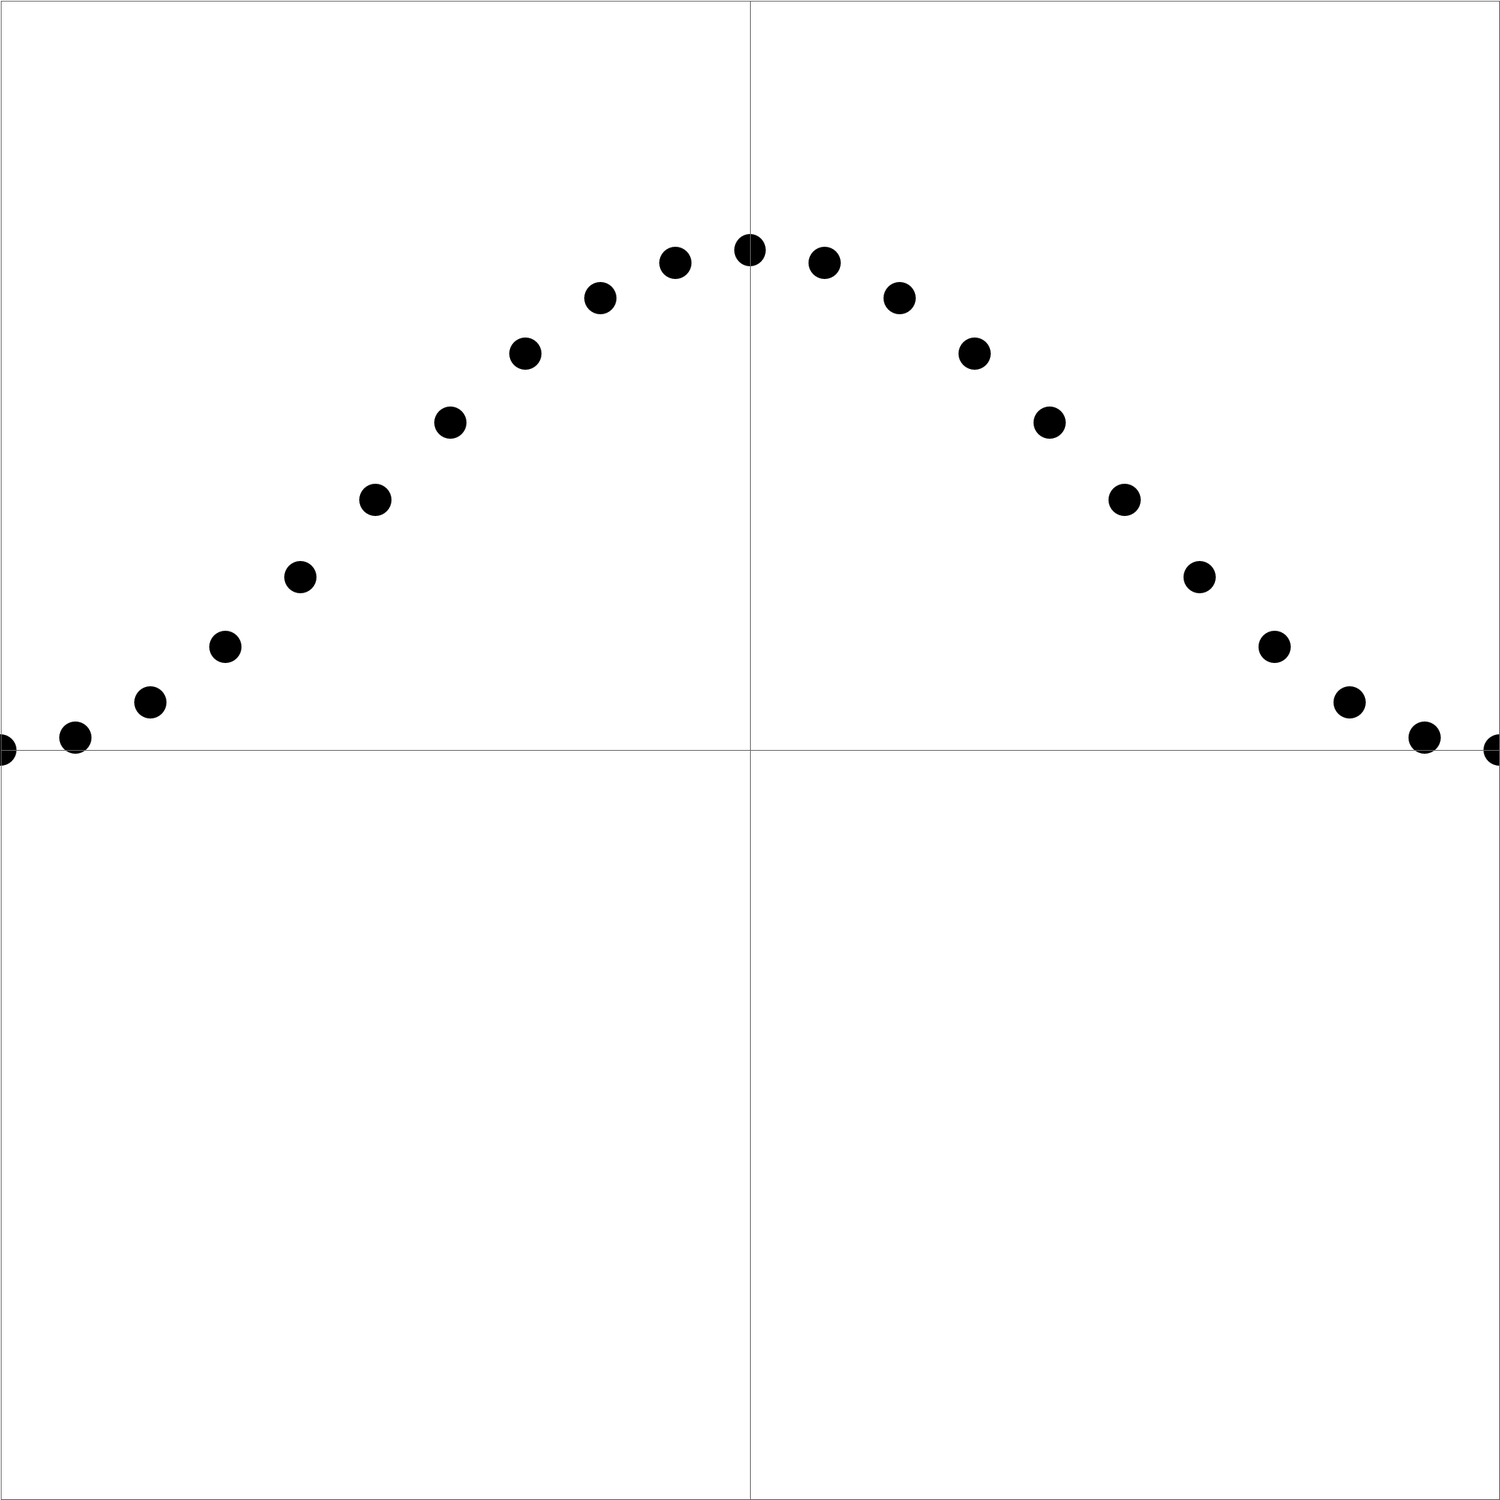
\includegraphics[width=\textwidth]{primer1_1}
				%\caption{D[Численное решение]}
				\label{fig:first}
			\end{minipage} {$\to$} (Label №1) $\to$\quad
			\begin{minipage}{0.35\textwidth}
				\centering
				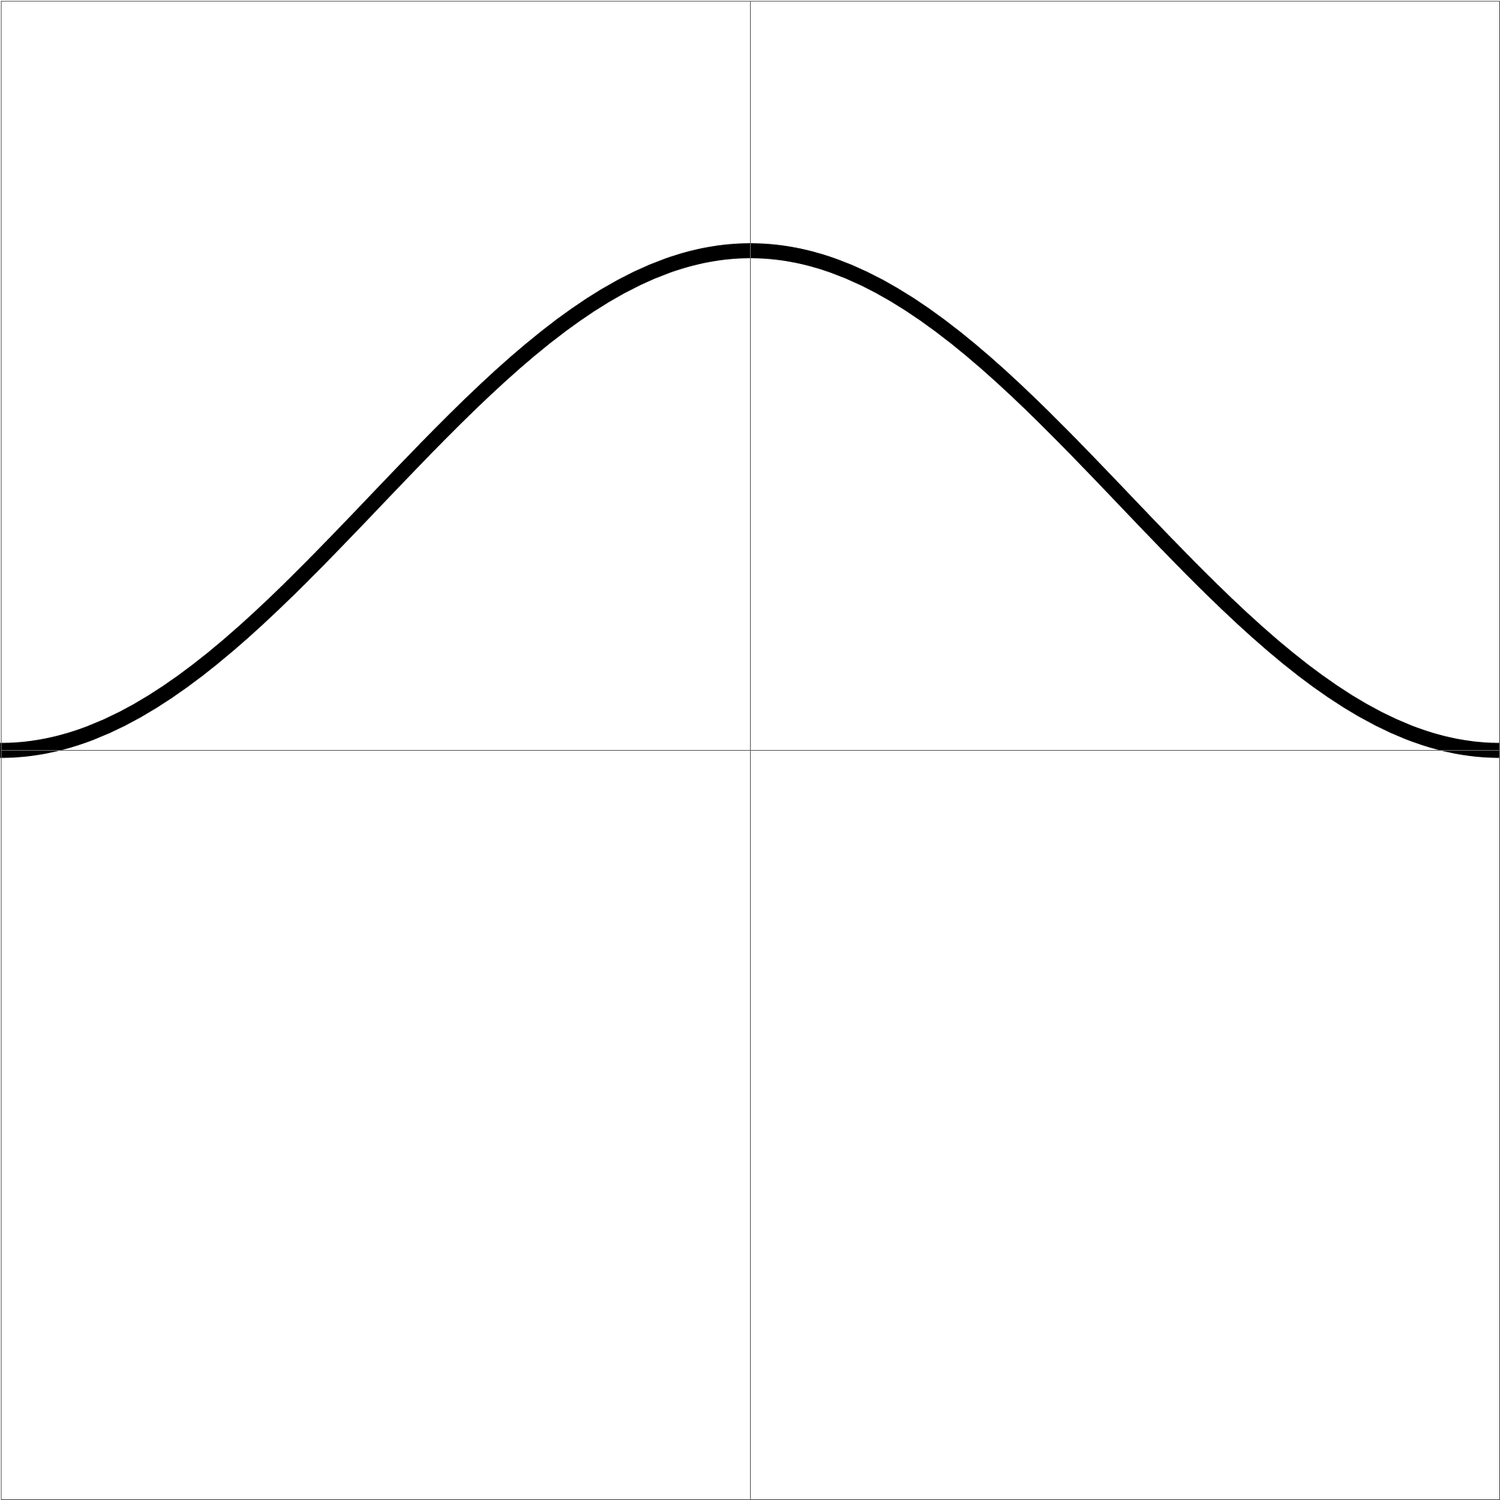
\includegraphics[width=\textwidth]{test4}
				%\caption{Улучшенное решение}
				\label{fig:second}
			\end{minipage}
		\end{figure}
\end{frame}

\section{Результаты работы программы улучшения решения}
\begin{frame}
\frametitle{Результаты работы программы улучшения решения}


\begin{table}[ht!]
	\caption{Результаты точности работы программы}
	\centering
	\adjustbox{scale=1}{%
	\begin{tabular}{|l|l|l|l|}
		\hline
		№ & Шаг по времени, $\tau$  & Шаг по пространству, $h$ & Точность , \%      \\ \hline
		\textbf{1}  & 0.1                    & 0.1    				   & 82          				\\ \hline
		\textbf{2}  & 0.05                   & 0.1   			       & 84         				\\ \hline
		\textbf{3}  & 0.05                   & 0.05   				   & 89        			    \\ \hline
		\textbf{4}  & 0.01     `			 & 0.01  				   & 93     					\\ \hline
	\end{tabular}}
\end{table}	
Стоит отметить, что результаты могут отличатся в зависимости от множества факторов, к которым относятся выбор коэффициентов сети, количество эпох обучения и особенности набора данных для обучения.
\end{frame}

\section{Заключение}

\begin{frame}
\frametitle{Заключение}
\begin{block}{}
	Таким образом в ходе работы
	\begin{enumerate}
		\item были изучены численные методы решения уравнения переноса, проведено тестирование численных методов на 5 тестах, а также созданы несколько программ. 
		\item Была создана программа, которая по неточному решения уравнения переноса возвращает точное. Была реализована программа на языке программирования С++17 для численного решения уравнения переноса различными схемами, а также реализованы 5 тестов. 
		\item  Реализована модель сверточной нейронной сети для распознавания решений уравнения на языке программирования Python 3.9.2 с помощью библиотеки машинного обучения TensorFlow 2.15.0.
	\end{enumerate} 
	
	Как итог, реализована программа, которая с помощью модели сети улучшает неточное решение данного уравнения до точного. 
\end{block}
\end{frame}




	
%\end{frame}
\end{document}